\subsubsection{Fragment modify form}

In fragment modify form the user could create a new fragment. In addition he could see the compared text passage with colors directly while adjusting the form as well. This feature was enabled by using an ajax function combining with an onchange-event in Javascript.

\begin{figure}[!h]
  \centering
  \fbox{
    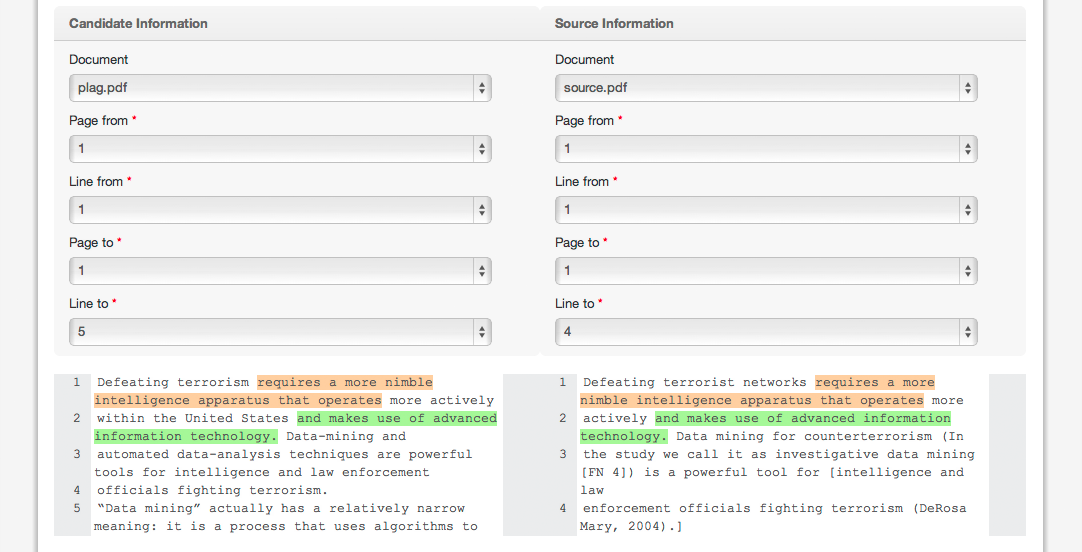
\includegraphics[width=0.97\textwidth]{images/fragment-form.png}
  }
  \caption{Text comparison function in fragment modify form}
  \label{fig:report_deckblatt}
\end{figure}

Here is the code in Jquery

\begin{lstlisting}[caption=Cropping an image to a square aspect ratio]
// executes a simtext comparison in fragment modify form
  function compareTexts() {
    if($("#candidateLineFrom").length != 0) {
      $.post("/document_page/compare", {
        candidateLineFrom: $("#candidateLineFrom").val(),
        candidateLineTo: $("#candidateLineTo").val(),
        sourceLineFrom: $("#sourceLineFrom").val(),
        sourceLineTo: $("#sourceLineTo").val(),
        highlight: true
      }, function(response) {
        if($('#candidateText').length == 0) {
          $('#fieldset-candidateGroup').append('<div id="candidateText" class="src-wrapper"/>');
          $('#fieldset-sourceGroup').append('<div id="sourceText" class="src-wrapper"/>');
        }
        $('#candidateText').html(response.data.plag);
        $('#sourceText').html(response.data.source);
      }, "json");
    }
    return false;
  }
  $("#candidateLineFrom, #candidateLineTo, #sourceLineFrom, #sourceLineTo").change(function(){
    compareTexts();
  });
  compareTexts();
\end{lstlisting}